\documentclass[10pt]{IEEEtran}
\usepackage[T1]{fontenc}
%\documentclass[12pt]{Article}
%\renewcommand\rmdefault{phv}
%\usepackage[doublespacing]{setspace}
%\usepackage[margin=1in]{geometry}
\usepackage{hyperref}
\usepackage{graphicx}
\usepackage[fleqn]{amsmath}
\usepackage{blindtext}
\usepackage{pgfplots}
\pgfplotsset{compat=1.9}
\usepackage{hyperref}
\usepackage{breakurl}
\usepackage{indentfirst}
\usepackage{authblk}
\PassOptionsToPackage{bookmarks=false}{hyperref}
\hypersetup{draft}
\usepackage{todonotes}
\usepackage{svg}
\usepackage{textcomp}
\usepackage{algorithmicx}
\usepackage[noend]{algpseudocode}
\usepackage{algorithm}
\newcommand*\Let[2]{\State #1 $\gets$ #2}
\newcommand*\Append[2]{\State #1$.append($#2$)$}
\providecommand{\myceil}[1]{\left \lceil #1 \right \rceil }
\tikzset{declare function={Ceil(\x)=round(\x+0.5);}}
\usepackage[backend=biber]{biblatex}
\addbibresource{ZTree.bib}
\usepackage{authblk}

\title{Sybil Resistant P2P Range Queries Over the Blockchain}
\author{Charles Noyes \\ cnoyes@usc.edu \\ Villa Park High School }
\date{\vspace{-5ex}}


\begin{document}
\maketitle

\begin{abstract}
We present the design of a novel data structure. We aim to solve the issue of window/range-based queries of distributed data stores in peer to peer architectures. Traditional models, for example, distributed hash tables (DHTs), are hostile towards window queries because their hashing operations are designed to uniformly distribute stored data across a defined key space; the hashing operations used to achieve this even key distribution inherently erase all characteristics of the target data that could be used to classify it. We solve this problem of erasure by defining a scheme in which higher-order data is mapped to a first-dimensional key space, while preserving locality. The resulting key space is not uniformly distributed, so we define a distributed consensus protocol in which participants in our network agree to target highly populated regions of the key space, through deterministic redistribution. This consensus scheme also provides protection from Sybil attacks, as it is a series of stratified hash-based proof-of-work systems. A peer to peer communication system acts as the underlying network for participants, providing all of the traditional benefits of a P2P architecture, while allowing our solution to operate reliably in the presence of adversaries.
\end{abstract}


\section{Notation}

\noindent Tuples/Lists: $[a,b,c,...]$

\noindent Application of a function $f$ to an input $x$: $y=f(x)$

\noindent Application of a hash function $H$ with $k$ output bits: $H_{k}(x) = \{0,1\}^{[k]}$

\noindent Keys of user $j$: $ PUBK_j; PRIVK_j $

 
\section{Introduction}
\par Decentralized networks, such as those used in the Bitcoin and Gnutella projects, have a need for data stores that are able to operate in hostile environments. Distributed hash tables are, arguably, the most widespread distributed data structure for these purposes~\cite{Stoica:2001dj,Rowstron:2001ea,Ratnasamy:2001wn}. They are used in many large-scale open-source projects~\cite{Freitas:2013tb,Xu:2010vs,Perfitt:2010fh} as the underlying infrastructure.

\par Simply put, DHTs were created to provide hash table-like functionality on an Internet-scale level~\cite{Ratnasamy:2001wn}. They expose basic PUT and GET requests (operating on <key,value> pairs) to clients, allowing them to store and retrieve information from the DHT. The difference between a hash table and a DHT is the scope of the mechanism: DHTs are able to operate in an entirely decentralized setting, where responsibility for the mapping of keys to values is distributed pseudo-uniformly among all participants in a P2P network. Notable networks that utilize DHTs include the Coral Content Distribution Network~\cite{Freedman:2004vb}, the Storm Botnet~\cite{Holz:2008uk}, and the BitTorrent file sharing protocol~\cite{Cohen:y1_8mBnw}.

\par Keys used in traditional DHTs are calculated using a hash function. Given that the digest (output) of a hash function is some number of bits, each with the same probability of being $'1'$ or $'0'$, it follows that the outputs will be randomly distributed within the hash function's key space~\cite{Stoica:2001dj}. This keyspace is the set of all possible outputs; for a hash function with $k$ output bits, this is the set $\{0,1\}^{[k]}$. Assuming that a given hash function's outputs are actually evenly distributed, one can mathematically verify even partitioning of the key space. The participants can thus trust that the load will be balanced fairly among all nodes. No one node will have complete control, and no group of nodes will be unfairly burdened due to their residing in some supposed 'hotspots' in the key space, in which a disproportionally high number of objects are stored.

\par All aforementioned systems use DHTs in an 'exact-match' lookup scenario; the even distribution of hash functions once again comes into play. The purging of any locality (that is, the property of alike object's digests being somehow as 'distant' from one another as the objects themselves) precludes range or window-based queries. According to Ramabhadran et al., "\textit{However, range queries, asking for all objects with values in a certain range, are particularly difficult to implement in DHTs. This is because DHTs use hashing to distribute keys uniformly and so can't rely on any structural properties of the key space, such as an ordering among keys}"~\cite{Ramabhadran:2004tr}\textit{.}

The idea of locality vs. evenness is fundamental to our work. Intuitively, locality is preserved for any given set of objects (serializable to a numeric representation in some fashion) $A,B,$ and $C$ in a function $f$ such that
\begin{equation} \label{eq:locality}
|A-B| < |B-C| \Rightarrow |f(A)-f(B)| < |f(B) - f(C)|,
\end{equation}
and traditional hash functions obviously do not fulfill this requirement.

\section{Related Work}
\par Some research has been done on the usage of a DHT as an overlay on top of a traditional data structure to enable range queries~\cite{Ramabhadran:2004tr,Desnoyers:2008uo,forestiero2009self}. However none of the currently proposed solutions are useful in a true P2P network. Sybil attacks, the orchestrated undermining or subversion of reputation or voting systems through the bulk forging of a identities in P2P networks, are arguably the most severe vulnerability in decentralized networks~\cite{Douceur:2002jr}. A litany of papers have been published on this attack in the context of DHTs (e.g.~\cite{LesniewskiLass:2010ue}), and yet the subject is not even broached in any of the cited works.


\section{Our Approach}
\begin{figure}[!t]
\centering
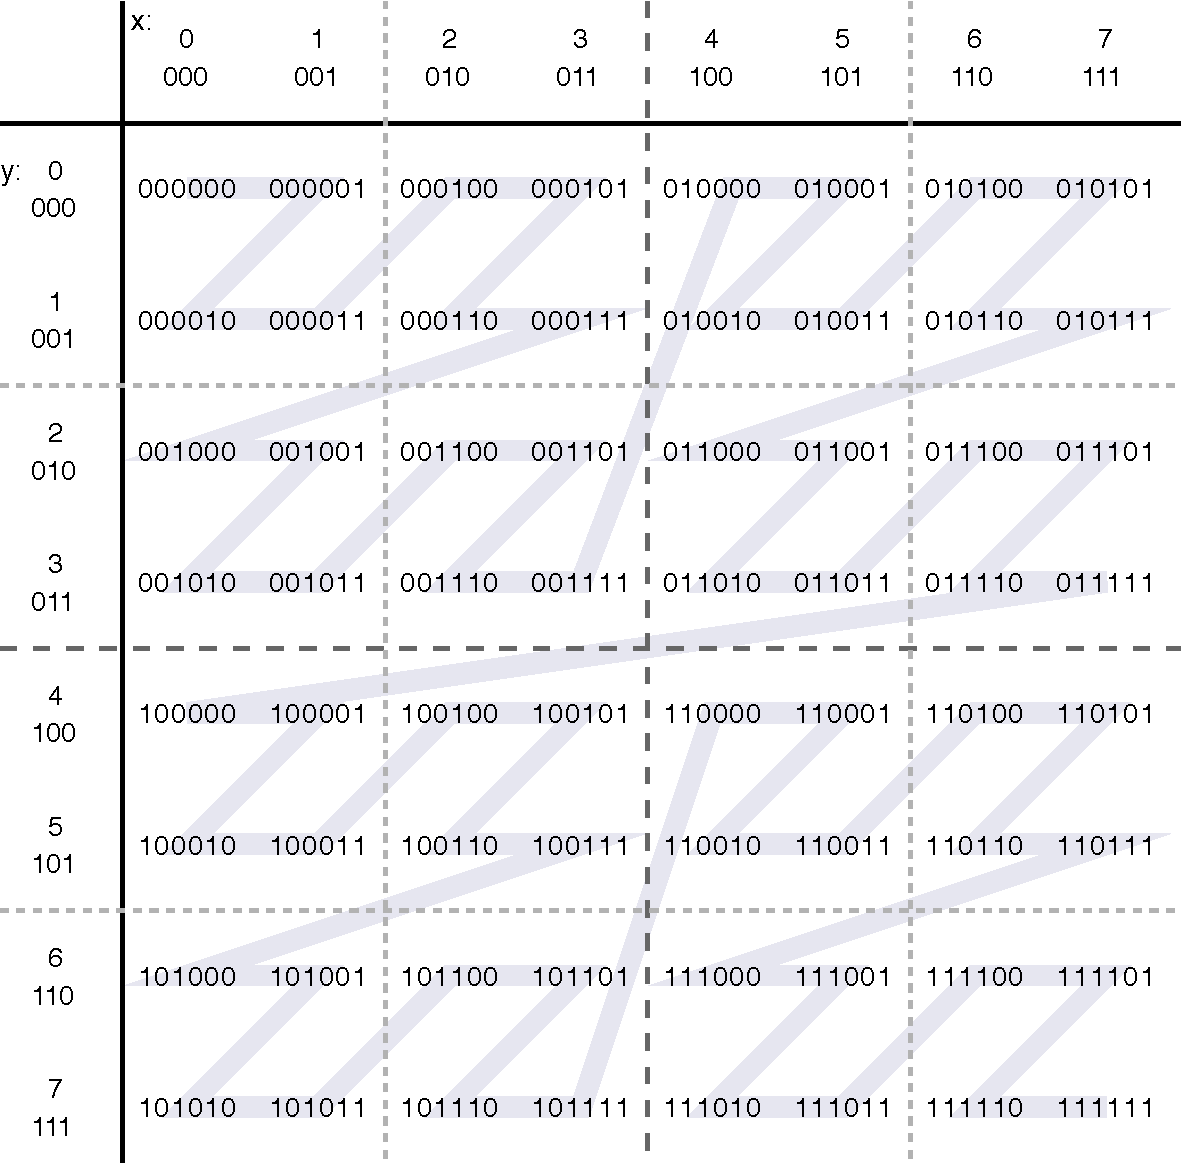
\includegraphics[width=3in]{ZCurve}
\caption{Z-Order Curving of the Integral Cartesian Plane~\cite{ZorderCurve:2015vo}}
\label{fig_MCode}
\end{figure}

\par The Squid project~\cite{Schmidt:2003cd}, another tangentially related work, has actually tried to define protocols for more generalized searching (e.g. range and keyword queries), in much the same way we have. The similarities end in the applicability of their work to situations that are not just distributed in a peer to peer network, but truly decentralized. The differences between the two are slight but of paramount importance to the applicability of a protocol that operates correctly only in the first case; it is relatively easy to distribute a process across a trusted network, but decentralization is another beast entirely.

\par A DHT that does work in a decentralized fashion would be enormously useful in a variety of settings. No data structure in existence has these capabilities and this work is, in fact, the direct result of the inability to find an existing solution. Some potential applications include scalable content addressable networks, decentralized applications, and sensor/information networks that potentially operate in the presence of adversaries.




\par We believe that the best solution is one in which we only slightly modify the way in which a DHT works. Substituting a space filling curve for a hash function would allow us to preserve locality of data in a DHT with defined limitations on what kind of data may be stored in it. A space filling curve brings its own set of limitations, however, and so we also present a few different approaches to mitigate those problems.

\subsection{Hash Function Replacement}

\par Currently, we believe that bit interleaving is a promising replacement for hash functions. Through the use of space filling curves, such as a Z-Order curve (sometimes called the Morton curve), $N$-dimensional data can be mapped to the first dimension (such that it may be stored in-memory). The mapping of a section of the integral Cartesian plane to binary, through the interleaving of the $x$ and $y$ coordinates, is illustrated in Fig.~\ref{fig_MCode}.

\par Interestingly, the interleaving of bits to form Morton codes preserves the locality of the initial data in the output, satisfying Eq.~\ref{eq:locality}. There is, however, no currently agreed upon scheme for the extension of this function to floating point numbers. A few solutions have been proposed, such as~\cite{Connor:2010eq}, but none have been truly validated. We do not believe this to be a significant obstacle, as imperfect solutions work well enough for the time being.

\par For now, we are using longitudinal and latitudinal coordinates to test range based searches in a sorted key-value database. Our algorithm to serialize the decimal coordinates to bytes is very simple. The coordinates $lat$ and $lon$ are multiplied by a constant, which is dependant on the size of the calculated Morton Code table (a large table allows for a larger constant, which in turn leads to a more accurate serialization), and converted to integers. Those integers are then fed into an algorithm that performs the operations show in Fig.~\ref{fig_MCode}.

\begin{figure}[!t]
\centering
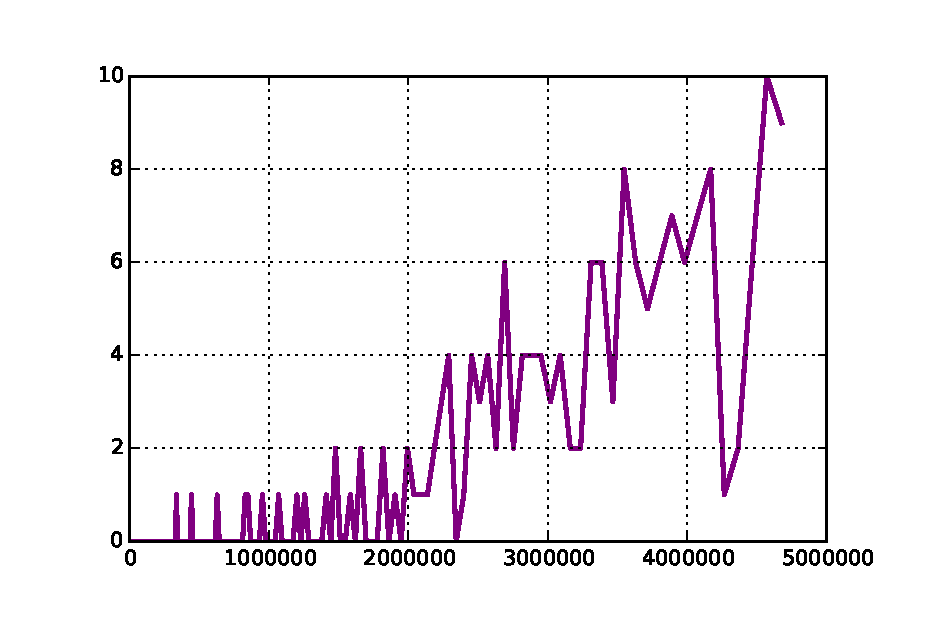
\includegraphics[width=3.5in]{errors.eps}
\caption{Floating Point Serialization Scheme Errors}
\label{fig_ZOrd}
\end{figure}

\par This is an imperfect solution, however the number of errors in a real-world test of this algorithm showed the error rate to be fairly negligible. To measure lookup accuracy on a large corpus, we performed a range query (the magnitude of the query was always the same) on random data sets of varying sizes, using the algorithm proposed above as our serialization scheme.
% \begin{algorithm}
%   \begin{algorithmic}[1]
%   \Require{A '/' denotes two variables with different prefixes, and is used to save line space.}
%   \vspace{-0.4cm}
%     \Statex
%     \Function{Test}{$n,min/maxLat,min/maxLon$}
%         \Let{$storageDic$}{$\{\}$}
%         \Let{$correctResults$}{$[]$}
%         \Let{$realResults$}{$[]$}
%         \For{$i \textrm{ in Range}(n)$}
%             \Let{$lat$}{$\textrm{RandFloat}(-90,90)$}
%             \Let{$lon$}{$\textrm{RandFloat}(-180,180)$}
%             \Let{$key$}{$Eq.$~\ref{eq:serialization}$(lat,lon)$}
%             \Let{$storageDic[key]$}{$i$}
%             \If{$(minLat<lat<maxLat)\&\&$ \par 
%             \hskip\algorithmicindent$(minLon<lon<maxLon)$}
%                 \Append{$correctResults$}{$i$}
%             \EndIf
%         \EndFor
%         \Let{$minCode$}{$Eq.~\ref{eq:serialization}(minLat/Lon)$}
%         \Let{$maxCode$}{$Eq.~\ref{eq:serialization}(maxLat/Lon)$}
%         \For{$key \textrm{ in } storageDic.keys()$}
%             \If{$minCode < key < maxCode$}
%                 \Append{$realResults$}{$key$}
%             \EndIf
%         \EndFor
%         \State \Return{$len(correctResults - realResults)$}
        
%     \EndFunction
%   \end{algorithmic}
% \end{algorithm}

\par Our results are shown in Fig.~\ref{fig_ZOrd}. We are confident that this decimal flooring scheme will effectively bridge the gap of time between the work we are doing here and the validation of a floating point-ready Z-Ordering scheme.

\begin{figure}[!t]
\centering
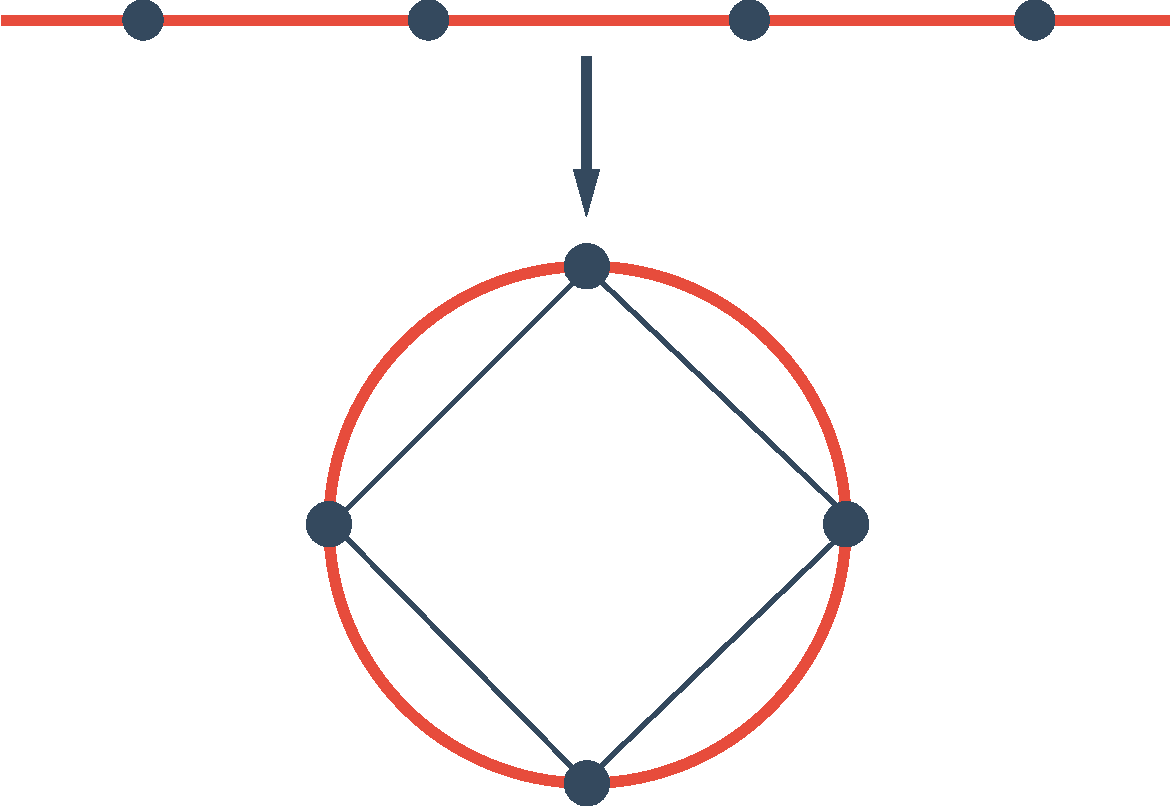
\includegraphics[width=3.5in]{finalRing}
\caption{Evenly Distributed Key Space Mapping}
\label{fig_kSpace}
\end{figure}

\subsection{Node Rearrangement}
\par Next, we come to the problem of key space distribution. Illustrated in Fig.~\ref{fig_kSpace} is the way in which we transform the linear version of the key space into a circular representation, and how the nodes communicate with their 'neighbors' in a DHT. On one 'end' of the linear representation is the lowest possible value (in binary, this would be the set $\{0\}^{[k]}$), and on the other is the maximum possible value ($\{1\}^{[k]}$). Notice that in both representations, the nodes are distributed evenly. Each occupies the same amount of space as the others, and together they cover the entire key space.

\par When using a Z-Ordering scheme as the key space location function, the mapped data almost certainly becomes highly 'clustered.' For example, when mapped to a binary keys pace, the global landline network shows a few highly populated regions, and oceans of nothingness between them. This is an unavoidable byproduct of the use of a locality-preserving function.

\par Fig.~\ref{fig_kSpaceUneven} shows a keyspace in which a locality preserving function was used, with red highlights gauging the fullness of each region in the key space. Notice that after the first transformation, two of the nodes are doing nearly all of the work, while the others have no load to bear. There is no existing mechanism for nodes to retroactively redistribute themselves, as shown in the second transformation.


\par We propose the inclusion of cryptographic proof-of-work, based on the Hashcash~\cite{Back:2002vq} model, with each stored piece of data. Because these proofs are difficult to compute, no entity can easily execute a Sybil-like attack against the rest of the network by including 'junk' proofs; all others would simply be able to see that the proofs are incorrect. A user $j$ would send this to the rest of the network:

\begin{figure}[!t]
\centering
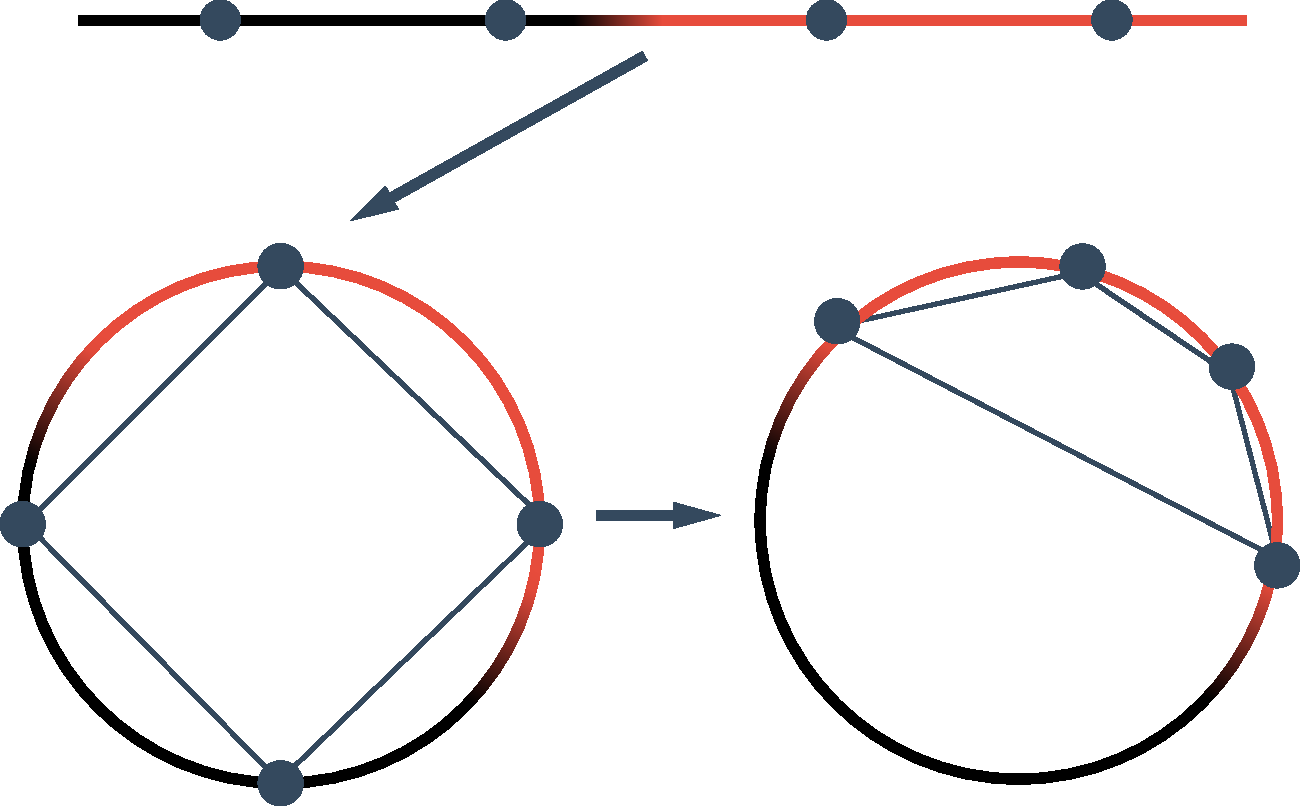
\includegraphics[width=3.5in]{unevenDistro}
\caption{Node Convergence}
\label{fig_kSpaceUneven}
\end{figure}

\begin{equation} \label{eq:proof}
SerializedData = [Data, Nonce],
\end{equation}

and then the validity of that proof is able to be verified in constant time simply by checking that $H(Data + Nonce)$ complies with the difficulty setting of the network.


\par When the nodes in a network wish to reconfigure themselves, all nodes are instructed to report all of the proofs-of-work they know about. All of the nodes then independently construct a curve of the key space density, such that they have some idea of 'saturation' in a given region, and attempt to converge onto more dense regions and away from sparsely populated regions.

\par From a game theory perspective, a proof-of-work system is greatly beneficial. Sybil attacks are largely mitigated, and there is no obvious advantage for a malicious node to withhold its knowledge of the proofs in its region. It does, however, introduce some amount of overheard into the network. We believe that this is not a terribly inhibiting factor, as the use cases for a decentralized (i.e. public) version of our data structure are almost always either altruistic or capitalistic in nature. To give an example of the former, folding@Home~\cite{Anderson:2002vr}, a network in which people donate unused computational resources to fold proteins, has been wildly successful. Bitcoin~\cite{Nakamoto:2008ti}, the decentralized P2P cryptocurrency network, is an excellent example of hashing power being used for the latter case. In both networks, there is no lack of available resources.

\par The actual methodologies of the 'reporting' and 'rearrangement' are left abstractly defined here intentionally. This is mostly because of the extreme variance between individual use cases; rarely will a generalized protocol work for all cases.

\section{Protocol Definitions/Analyses}
\subsection{Mitigation of Sybil Attacks on The DHT Proper}
\par Some of the claims made thus far are provable without the need for real-world trials. For example, we assert that Sybil attacks are mitigated through a proof-of-work system and that this work is not a growth inhibiting factor. Our proof-of-work system is a basic one, modeled on the HashCash~\cite{Back:2002vq} system. We define a 'proof' as being the value resulting of the inputting of both information and a random number to a hash function. If this proof meets the threshold of difficulty set by the network, it is accepted as valid. To show this, we assume that for a hash function of k bits, the set of possible results is exactly $\{0,1\}^{[k]}$. The odds of any $k'th$ bit being $0$ or $1$ are exactly even (in this case, $1:1$). Thus, the odds of the first $n$ bits being set to 0 is exactly $\frac{1}{2^n}$. Note that simply using $0$-prefixing as the method of work determination is simplistic, and 'better' schemes (like that of Bitcoin, which uses full hex values) can provide finer control. 

\par When applied to our data structure, we would be using the number of votes as our difficulty determining factor. The difficulty should be proportionate to the number of votes and dependant on some predefined ratio of necessary goodness (generally this will be $ > 50\%$, as a result of the Byzantine generals problem's limits in the general case). Mathematically,
\begin{gather}
z = \myceil{log_2{ (\frac{2^n}{\frac{N}{m}})}} \Rightarrow q = 2^z
\end{gather}
where $N$ is the population size, $m$ is the proportion of wanted goodness, $n$ is the maximum difficulty, $q$ is the average number of tries, and $z$ is the number of required leading $0$ bits.

\begin{figure}
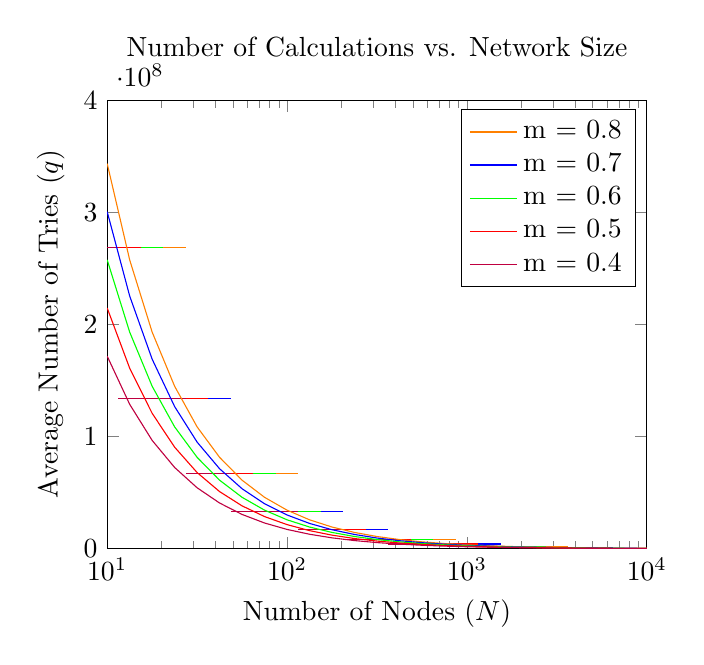
\begin{tikzpicture}
\begin{semilogxaxis}[
    jump mark mid,
    domain=10:10000,
    xmin = 10,
    xmax = 10000,
    ymin = 0,
    ymax = (0.4 * 10^9),
    title = {Number of Calculations vs. Network Size},
    xlabel = {Number of Nodes ($N$)},
    ylabel = {Average Number of Tries ($q$)},
    title style={yshift=1.5ex}
    ]
\addplot[color=orange]{2^(Ceil(ln((4294967296) / (x / 0.8))/ln(2)))};
\addplot[color=blue]{2^(Ceil(ln((4294967296) / (x / 0.7))/ln(2)))};
\addplot[color=green]{2^(Ceil(ln((4294967296) / (x / 0.6))/ln(2)))};
\addplot[color=red]{2^(Ceil(ln((4294967296) / (x / 0.5))/ln(2)))};
\addplot[color=purple]{2^(Ceil(ln((4294967296) / (x / 0.4))/ln(2)))};
\legend{m = 0.8,m = 0.7, m = 0.6,m = 0.5,m = 0.4}
\end{semilogxaxis}
\begin{semilogxaxis}[
    domain=10:10000,
    xmin = 10,
    xmax = 10000,
    ymin = 0,
    ymax = (0.4 * 10^9),
    yticklabels={,,},
    xticklabels={,,},
    hide axis
    ]
\addplot[color=orange]{(4294967296) / (x / 0.8)};
\addplot[color=blue]{(4294967296) / (x / 0.7)};
\addplot[color=green]{(4294967296) / (x / 0.6)};
\addplot[color=red]{(4294967296) / (x / 0.5)};
\addplot[color=purple]{(4294967296) / (x / 0.4)};
\end{semilogxaxis}

\end{tikzpicture}
\caption{Scaling Validation}
\label{fig_tryGraph}
\end{figure}

\par A reference graph for $n = 32$ is shown in Fig.~\ref{fig_tryGraph}, highlighting the relation between goodness thresholds ($m$) and the average number of hash calculations needed to find a good nonce ($q$), along varying network sizes ($N$). The lines with a ceiling function applied are those that would use only $0$-bit prefixing, whereas the continuous lines are those that would use an ideal scheme (even hex values are not truly continuous, but there are many more 'steps'). Illustrated is the proof of Sybil mitigation, as a result of proper proof-of-work scaling.

\par In a network with $100,000$ participants, the number malicious 'votes' that must be cast is $ > \frac{100000}{m}$. So, when $m = 0.5$ and $n = 50$, a normal user will have to calculate (about) $5.6\times{}10^8$ hashes to find a good nonce. Note that $n = 50$ is a more realistic baseline than $n = 32$. With a hash rate of $500KH/s$ and a wattage of of $650W$, reasonable empirical estimates of the hash rate and wattage of an average computer, it would take approximately $180$ seconds to find a nonce, or less than $1$\textcent. However, for an attack attempting to breach the consensus threshold $m$ of the network, it would take over $10,000$ hours or over $\$750$. Note that the price of electricity is estimated at $12\textcent$ per kilowatt-hour. 

\par One notable feature of our scheme is that the amount of power necessary to overcome the network is a constant (i.e. does not intrinsically rely on the size of $N$). Because we are decreasing the amount of work required from each new vote based on the current amount, the requisite amount of power required to overcome the rest of the network is decreased at the same rate. We include the term $\frac{N}{m}$ because it is possible to scale the amount of work required disproportionately, such that the rate of descent of the required work approaches $0$ logarithmically as $N \to \infty$.

\par For networks that are to be used only in the short term, are large but run on devices without much computational power, or that would benefit more from a lower barrier to entry than would be allowed for with linear scaling of the hashing requirements, our scheme works best. Many autonomous networks fit this set of criteria, and for those that don't, a system where the required work is not dependant on the present work can be used. Hybrid systems, for example ones in which the requisite work does not scale perfectly with the theoretical amount of work required for a Sybil attack overcoming $m$, are also very viable. There are really an endless number of possibilities, and our approach is presented here because no other scheme presents a working scaled difficulty model.


\subsection{Active Node Rearrangement}

\par We present here one possible methodology for a node rearrangement scheme. Approaches such as Self-Chord~\cite{forestiero2009self} have defined schemes similar to ours, with the notable absence of a method of fault tolerance in the face of adversaries. All other approaches are predicated on the idea that node rearrangement must be done by individual clients, using only the information at hand. These types of systems are inherently flawed, as local-optimum algorithms often fail in the face of higher level consensus attacks.

\par Our focus thus shifts to the problem of globalizing the knowledge scope of the network, such that individual nodes are not operating on disparate levels of information. A blockchain is used here, as it provides both a decentralized ledger-like data store, and an inherent higher-level consensus scheme ~\cite{Nakamoto:2008ti}. Our blockchain is modeled after that of Twister~\cite{Freitas:2013tb}; traditional cryptocurrency transactions are coupled with 'information blocks,' which are every $k'th$ block for some interval $k$.

\par The mechanics of the blockchain are well documented, so suffice to say that our variant leaves us with a working global knowledge scope; that is, all nodes in the network have access to whatever information the protocol defines as being needed on a network-wide scale. The difference between this scheme and a more simple one, e.g. P2P reporting via direct peer communication, is that the the hashing operations that extend the chain serve to 'validate' one branch, so nodes are assuredly operating on the same information. In the direct communication scenario, it is likely that nodes are operating on wildly disparate levels of information. Because of this, no global operations that rely on absolute canonicity of information (like hashing operations) can be used in those protocols, whereas the use of the blockchain allows us to assume the exact alikeness of nodes' knowledge scopes.

\subsubsection{Local-Optimum Rearrangement}

\begin{figure}
\centering
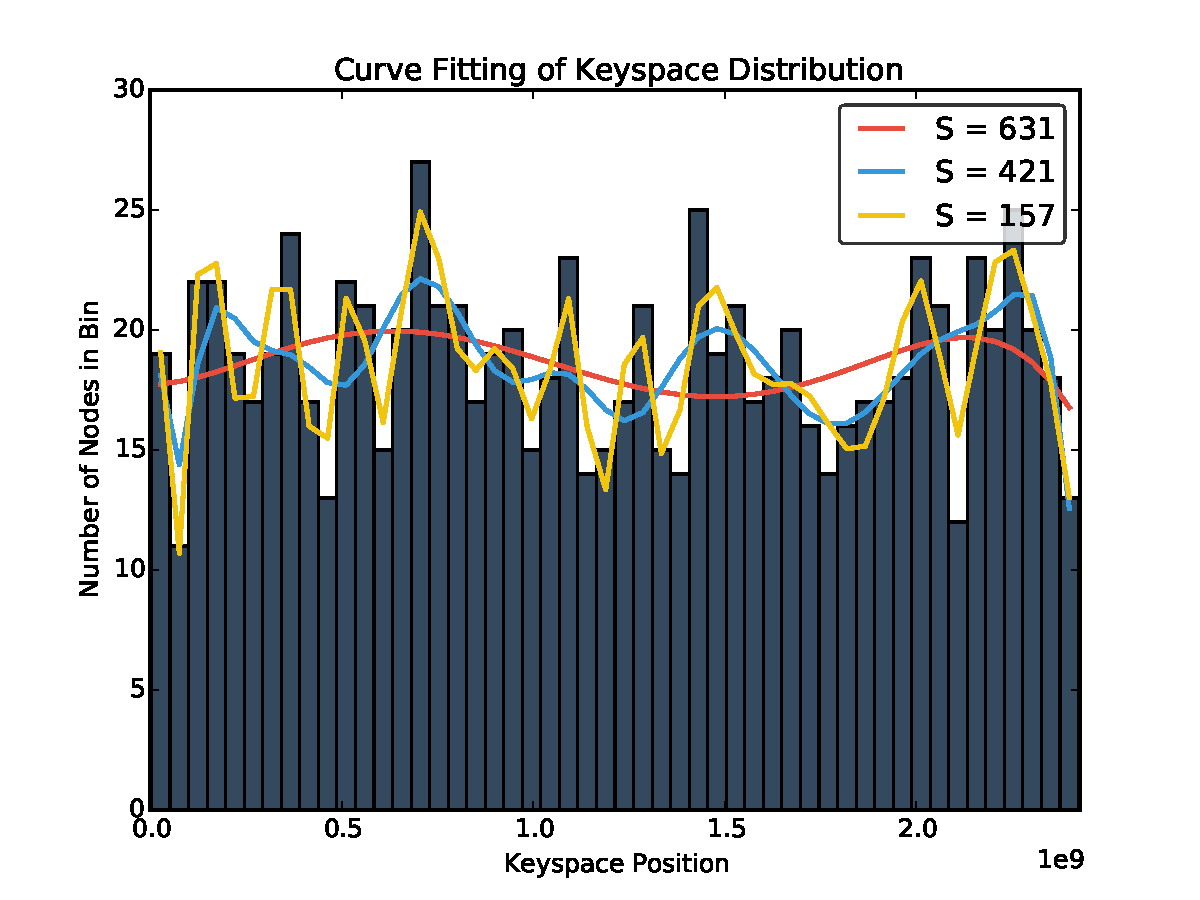
\includegraphics[width=0.5\textwidth]{plots/histogram}
\caption{Keyspace Histogram}
\label{fig:Histo}
\end{figure}
\par An easy solution to node convergence is to have individual nodes distribute themselves normally (i.e. through consistent hashing), and then use some metric of local density to have them move slightly in a favorable direction. This is very similar to the referenced projects using local-optimum algorithms (e.g. \cite{forestiero2009self}), but in our network there can be a bit more fine control. Illustrated in Fig.~\ref{fig:Histo} is a keyspace density histogram, fitted with splines of varying smoothness. It would be relatively trivial to have nodes perform some kind of binning operation, such as k-means clustering, to divide the keyspace into regions of distinct densities. They would then just evaluate their position in the keyspace, and move slightly in the direction of increasing density. In essence they would be normalizing their position in the keyspace, by some movement metric, to the nearest local maxima. 


\subsubsection{Global-Optimum Rearrangement}
\par A more perfect solution is to (verifiably) evenly distribute information to all known nodes. This requires that both all of the data and all of the nodes in the network be explicitly enumerated before rearrangement. As discussed earlier, we do this through the use of a blockchain. For example, suppose $Block_k$ contains all of the known data (similarly to how a torrent file works on the BitTorrent network), or in our case, all of the known proofs and their corresponding keyspace locations, for the time period proceeding that of $Block_{k-1}$. For $p$ proof's locations, each node takes the data from $Block_k$ to form a list $proofs[0,\dots{},p]$. $Block_{k+1}$ then enumerates all nodes that report a willingness to participate in this period of operation, and all nodes use that data to independently construct a list $nodes[0,\dots ,N]$.  


\par The list $proofs$ is then sorted according to the linear distance from the lowest proof location. $node$ is also sorted, somewhat cleverly. Each entry in $nodes$, $0\dots{}p$, is hashed together with $H(Block_{k+1})$. These new values are randomized in that no node other than the publisher of $Block_{k+1}$ could have known the value hash of the block, and thus neither the value of $H(node[0,\dots{},p] + H(Block_{k+1}))$. It follows that reliable subversion (i.e. subversion for more than a single chronological network period) would require a blockchain consensus-breaking exploit. 

\par The assigning of data to individual nodes is now trivial. Multiple protocols can work here, e.g. ones that overlap responsibility for fault tolerance, but a very simple reference is a decent enough proof of concept. The number of elements in $proosf$, $\lambda$, is divided by the number of nodes, $\sigma$, and converted to an integer $\lfloor{}\tau{}\rfloor{}$ that defines the number of data items assigned per node. Note that the number of unevenly distributed items as a result of rounding $\tau$ is simply  $\lambda \mod (\tau * \sigma)$. We now simply by traverse over all peers in $nodes$ and assign $\tau$ $proofs$ per node. 
\begin{figure}

\centering
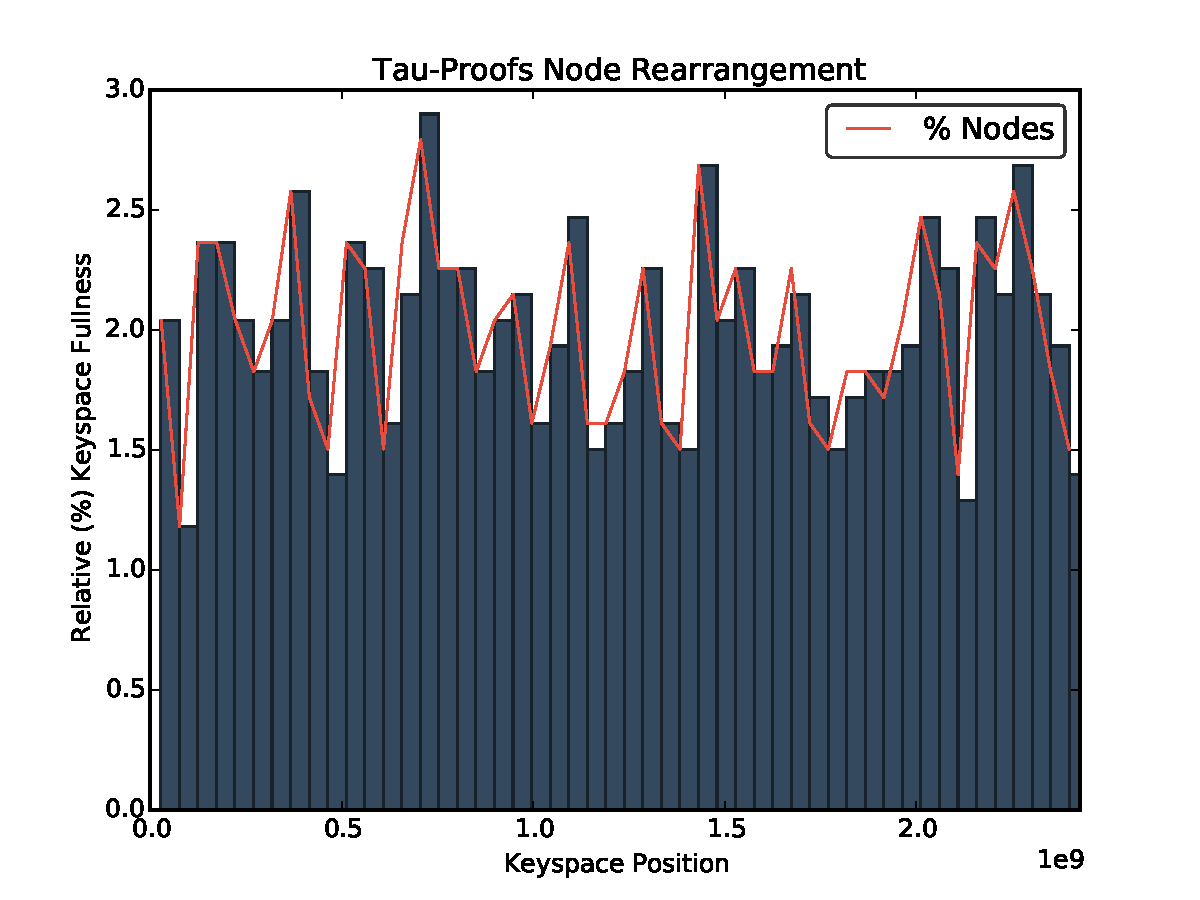
\includegraphics[width=0.5\textwidth]{plots/histogram_tau}
\caption{Results of Global-Optimum Rearrangement Test}
\label{fig:Histo2}
\end{figure}

\par Finally, our seminal results are shown in Fig.~\ref{fig:Histo2}. Notice the extremely close correlation between $\%$ keyspace fullness of items and of nodes. We calculated an average error rate of $0.4\%$ (p < $0.01$). Thus, we can confidently conclude that our solution works, completely. Many of the ideas introduced in this paper were novel, but this result represents the culmination of all of them. It is an entirely novel, unexplored scheme, that works completely. We have successfully created a range-queryable distributed data structure that can operate in the presence of adversaries, and are the first ones to have done so; no other work has ever been able to make this claim.

\section{Conclusions}
\par A working decentralized, distributed, range-querayable data structure has wide reaching implications for multiparty computation schemes. Things like decentralized autonomous sensornets are made a very real possibility. The number of applications in ecosystems like the Bitcoin network are veritably endless.

\par Our results unequivocally showed the success of this project. Our proposed data structure is able to operate in the presence of adversaries, while introducing minimal overhead to the legitmate network participants. Our results are supported by the marginal advances made by several previously conducted studies (e.g. \cite{forestiero2009self,Freitas:2013tb,LesniewskiLass:2010ue}). Note, however, that all of those referenced studies focused on disparate problems, and their solutions are not reconcilable. That is, the formulation of a master data structure that incorporates the granular improvements proposed in each of those works would not be a viable data structure.

\par In the future, one very interesting area of possible exploration is the speed that our data structure allows for. Because of the globalized knowledge scheme, it is likely that the average lookup complexity is $\mathcal{O}(1)$, due to the fact that all positions are known at all times. The proof is still in revision, but the assumption follows from the known value of a normal hash table ($\mathcal{O}(1)$). In a normal hash table, the location of storage in memory is 'constant' in that no network query must be done to know it. In our network, the query is a lookup on disk of that location in the keyspace (from our blockchain's database), and thus is not dependent on the knowledge of peers in a node's table of relationships (as is the case in~\cite{Stoica:2001dj}). There is, however, the problem of churn, peers entering or exiting the system constantly, and this is something that must be taken into consideration, since our current node rearrangement scheme relies on the assumption that a majority of nodes will remain in the system for the duration of a given network interval. 




\printbibliography
\end{document}
